As previously mentioned, each video has its own characteristics and challenges, yet there are two main goals they all share.
The first is to include all the foreground pixels in the foreground image, and the second is to exclude as many background pixels as possible from the foreground image. \\
For example figure~\ref{fig:problematic-frame} shows a problematic frame from the swan video.
Notice the two marked spots, unfortunately, the tip of the swans head is excluded from the foreground image and a spot in the reflection of the swan in the water is included.
In order to fix that, achieve our goal and result in an overall better performance, there are several components we can tune in our method.
\begin{figure}
    \centering
    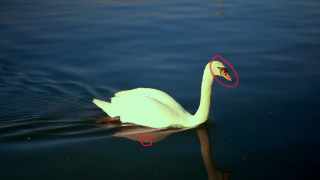
\includegraphics[scale=1.8]{images/swan/example}
    \caption{problematic frame}
    \label{fig:problematic-frame}
\end{figure}

\subsection{Including X and Y}\label{subsec:xy}
The first thing we can do is to include X and Y coordinates of each pixel in the models train data.
This should result in a better clustering process, as the pixels will be clustered not only by their color but also by their location.
The coordinates are normalized to the range [0,1] and concatenated to the color values.
If we get more accurate clusters from each model, we should get a better separation overall.
\subsection{Defining The Prior}\label{subsec:prior}
The third thing we can do is to better define the prior given to the models as input.
If we use a NIW prior, we can better customize it to fit each model.
The NIW prior is defined by the following parameters:
\begin{itemize}
    \item $\mu$ - the mean of the distribution.
    \item $\kappa$ - how much to weight the prior mean.
    \item $\nu$ - the degrees of freedom.
    \item $\phi$ - the covariance matrix.
\end{itemize}
So if we adjust these parameters according to our initial input, we can get models that better fit our data.
For each model we will use the first frame mean and covariance as \texttt{$\mu$} and \texttt{$\phi$} respectively.
$\kappa$ and $\nu$ will be set according to how much we trust our mean and covariance.
The resulting models should be better and the output gaussian mixtures should be more accurate.
\pagebreak
\subsection{Decision Rule}\label{subsec:decision}
The second thing we can do is to better define the decision rule that determines whether a pixel is foreground or background.
The simple approach is for a given pixel, calculate the probability of it belonging to each cluster and assign it to the part the cluster with the highest probability belongs to.
This approach is not wrong, but it is not optimal, as there could be situations where it would classify badly.
For instance, the probability of a pixel belonging to a single cluster in the foreground is high, but the weighted sum of probabilities of clusters in the background is much higher.
This is where a gaussian mixture would come in handy as its pdf function would classify that pixel to the background.
Yet this change did not improve the results significantly, so lets consider another case.
Consider a pixel that its probability of belonging to the foreground and background are almost equal, plus it is quite low.
We would probably be better off not classifying it in the foreground, since the foreground is usually much smaller than the background,
meaning the probability of it being in the background is probably richer as it is affected by more clusters.
This is where the threshold comes in, we can set a threshold for the probability of a pixel belonging to the foreground,
and if it is lower than that and quite close to the probability of the background, we will classify it as background.
The rule is implemented in \texttt{\_is\_pixel\_in\_object} method in \textcolor{red}{video\_object\_segmentation.py} file.
\lstinputlisting[language=Python, firstline=122, lastline=128,label={lst:pixel-in}]{../video_object_segmentation.py}
This change affects the results significantly, as now we are stricter with the pixels we classify as foreground.
So we get less false positives but also a bit less true positives that we will need to address.

\subsection{Model Adjustment}\label{subsec:model}
The last component we will address is the model adjustment.
At each iteration, after segmenting the foreground and background, we input the new images to the models and let it run a few iterations, resulting in improved gaussian mixtures.
The question is how many iterations should we run?
Intuitively, we would want to run as many iterations as possible, to let the models converge.
But the models also have a decay factor, meaning that the more iterations we run, the more the models will forget their previous inputs.
Our ground truth is the first frame, so we would want the models to remember it as much as possible, too many iterations will make the models forget it.
So we need to find a balance between the two, reducing the number of iterations at each frame to between 3 and 5 iterations, should result in better models.